\documentclass[nofootinbib,aps,prd,preprint,superscriptaddress]{revtex4}
\usepackage{amsmath,graphicx,hyperref}
\usepackage{slashed}
\usepackage{epstopdf}


%%%%%%%%%%%%%%%%%%%%%%%%%%%%%%%%%%%%%%%%%%%%%%%%%%%%%%%%%%%%%%%%%%%%%%
%%%%%%%%%%%%%%%%%%%%%%%%%%%%% Command %%%%%%%%%%%%%%%%%%%%%%%%%%%%%%%%
%%%%%%%%%%%%%%%%%%%%%%%%%%%%%%%%%%%%%%%%%%%%%%%%%%%%%%%%%%%%%%%%%%%%%%

\newcommand{\fms}[1]{{#1}\!\!\!/}
\newcommand{\fmsl}[1]{{#1}\!\!\!\!/}

\newcommand{\mc}{\mathcal}
\newcommand{\mr}{\mathrm}
\newcommand{\mP}{\mathcal{P}}
\newcommand{\mO}{\mathcal{O}}

\newcommand{\be}{\begin{equation}} 
\newcommand{\ee}{\end{equation}} 
\newcommand{\beq}{\begin{equation}} 
\newcommand{\eeq}{\end{equation}} 
\newcommand{\bea}{\begin{eqnarray}} 
\newcommand{\eea}{\end{eqnarray}} 

\newcommand{\ov}{\overline}
\newcommand{\pp}{\perp}
\newcommand{\dg}{\dagger}
\newcommand{\n}{\overline{n}}
\newcommand{\nn}{\frac{\fms{\overline{n}}}{2}} 
\newcommand{\nnn}{\frac{\fms{n}}{2}} 

\newcommand{\bl}[1]{{\bf{#1}}}
\newcommand{\bla}[1]{|{\bf{#1}}|}
\newcommand{\blp}[1]{{\bf{#1}}_{\perp}}
\newcommand{\blpu}[1]{{\bf{#1}}^{\perp}}
\newcommand{\blpa}[1]{|{\bf{#1}}_{\perp}|}
\newcommand{\bs}[1]{\boldsymbol{#1}}
\newcommand{\bsp}[1]{{\boldsymbol{#1}}_{\perp}}

\newcommand{\ds}{\displaystyle} 
\newcommand{\nnb}{\nonumber} 

\newcommand{\as}{\alpha_s} 

\newcommand{\eps}{\epsilon} 
\newcommand{\veps}{\varepsilon} 

\newcommand{\UV}{\veps_{\mr{UV}}}
\newcommand{\IR}{\veps_{\mr{IR}}}

\newcommand{\La}{\Lambda^2_{\rm{alg}}}



%%%%%%%%%%%%%%%%%%%%%%%%%%%%%%%%%%%%%%%%%%%%%%%%%%%%%%%%%%%%%%%%%%%%%%

%\topmargin 0.0 in

\begin{document}

\baselineskip 3.0ex 

\vspace*{18pt}

%%%%%%%%%%%%%%%%%%%%%%%%%%%%%%%%%%%%%%%%%%%%%%%%%%%%%%%%%%%%%%%%%%%%%%
%%%%%%%%%%%%%%%%%%%%%%%%%%%%% Title %%%%%%%%%%%%%%%%%%%%%%%%%%%%%%%%%%
%%%%%%%%%%%%%%%%%%%%%%%%%%%%%%%%%%%%%%%%%%%%%%%%%%%%%%%%%%%%%%%%%%%%%%

\title{Title?}

\def\Pitt{Pittsburgh Particle Physics Astrophysics and Cosmology Center (PITT PACC) \\ Department of Physics and Astronomy, University of Pittsburgh, Pittsburgh, Pennsylvania 15260, USA}

\author{Cameron Mahoney}
\email[E-mail:]{cbm34@pitt.edu}
\affiliation{\Pitt}
\author{Adam K. Leibovich}
\email[E-mail:]{akl2@pitt.edu}
\affiliation{\Pitt}
\author{Andrew R. Zentner}
\email[E-mail:]{zentner@pitt.edu}
\affiliation{\Pitt}  

\begin{abstract} 
\baselineskip 3.0ex   
Abstract?
\end{abstract}

\maketitle 

%%%%%%%%%%%%%%%%%%%%%%%%%%%%%%%%%%%%%%%%%%%%%%%%%%%%%%%%%%%%%%%%%%%%%%

\section{Introduction}



\section{Computational details}
	The process we are considering, the bremsstrahlung of a dark photon from nucleon-nucleon scattering, is similar in many ways to the classic calculation of axion emission from supernova cooling. The differences arise due to the mass of the dark photon, which can be on the order of the temperature of the supernova.  This leads to different kinematics compared to the axion case.  However, the calculation roughly follows the analogous calculation for axions, as laid out by Raffelt, which we briefly review below.  As in the classical axion calculation, we will use the one-pion exchange (OPE) approximation.  
	
\subsection{Bremsstrahlung amplitude calculation}
	 There are two processes to consider: the $pp$ scattering with the bremsstrahlung of the dark photon, $ p+p \rightarrow p+p+A$, and the $pn$ scattering with bremsstrahlung, $ p+n \rightarrow p+n+A\ $. For the $pp$ case there are eight tree-level diagrams, with the emission of the $A'$ from each of the external legs, as shown in Fig. , while for the $pn$ case there are five diagrams, including when the $A'$ is emitted from the exchanged charged pion, as shown in Fig. .
	
The calculation of these diagrams are straightforward, using standard Feynman rules.  Each of the $p-p-\pi $ vertices contribute a factor of $g_{pp}$,  the pseudoscalar pion-nucleon coupling. $f_{pp}$, the pseudovector pion-nucleon coupling, is related by $g_{pp} = \frac{2M_N}{m_\pi} f_{pp} $. The $ p-p-A' $ vertex contributes $e\epsilon \gamma_\mu$, where $\epsilon$ is the mixing strength between the photon and dark photon. Labeling the contributions according to the Feynman diagrams in Fig. , the matrix elements are 
\bea
M_1 &=& \frac{4 M_N}{ m_\pi} \frac{f_{pp}^2 e \epsilon}{l^2-m_\pi^2
	 	}  \frac{1}{m_{A^\prime}^2 - 2 q_a \cdot p_1} \bar{u}(p_3) \gamma_5 u(p_2) \bar{u}(p4) \gamma_5 (\slashed{p}_1 - q_a +M_N)\slashed{\varepsilon} u(p_1),\\
M_2 &=& \frac{4 M_N}{ m_\pi} \frac{f_{pp}^2 e \epsilon}{k^2-m_\pi^2
	 	}  \frac{1}{m_{A^\prime}^2 - 2 q_a \cdot p_1} \bar{u}(p_4) \gamma_5 u(p_2) \bar{u}(p3) \gamma_5 (\slashed{p}_1 - q_a +M_N)\slashed \varepsilon  u(p_1), \\
M_3 &=& \frac{4 M_N}{ m_\pi} \frac{f_{pp}^2 e \epsilon}{l^2-m_\pi^2
	 	}  \frac{1}{m_{A^\prime}^2 - 2 q_a \cdot p_2} \bar{u}(p_3) \gamma_5 u(p_1) \bar{u}(p4) \gamma_5 (\slashed{p}_2 - q_a +M_N)\slashed \varepsilon  u(p_2), \\
M_4 &=& \frac{4 M_N}{ m_\pi} \frac{f_{pp}^2 e \epsilon}{k^2-m_\pi^2
	 	}  \frac{1}{m_{A^\prime}^2 - 2 q_a \cdot p_2} \bar{u}(p_4) \gamma_5 u(p_1) \bar{u}(p3) \gamma_5 (\slashed{p}_2 - q_a +M_N)\slashed \varepsilon  u(p_2), \\
M_5 &=& \frac{4 M_N}{ m_\pi} \frac{f_{pp}^2 e \epsilon}{l^2-m_\pi^2
			 }  \frac{1}{m_{A^\prime}^2 + 2 q_a \cdot p_3} \bar{u}(p_4) \gamma_5 u(p_1) \bar{u}(p3) \slashed{\varepsilon} (\slashed{p}_3 + q_a +M_N)\gamma_5 u(p_2),\\
M_6 &=& \frac{4 M_N}{ m_\pi} \frac{f_{pp}^2 e \epsilon}{k^2-m_\pi^2
		 		 }  \frac{1}{m_{A^\prime}^2 + 2 q_a \cdot p_3} \bar{u}(p_3) \gamma_5 u(p_1) \bar{u}(p4) \slashed{\varepsilon} (\slashed{p}_3 + q_a +M_N)\gamma_5 u(p_2),\\
M_7 &=& \frac{4 M_N}{ m_\pi} \frac{f_{pp}^2 e \epsilon}{l^2-m_\pi^2
		 		 }  \frac{1}{m_{A^\prime}^2 + 2 q_a \cdot p_4} \bar{u}(p_3) \gamma_5 u(p_2) \bar{u}(p4) \slashed{\varepsilon} (\slashed{p}_4 + q_a +M_N)\gamma_5 u(p_1),\\
M_8 &=& \frac{4 M_N}{ m_\pi} \frac{f_{pp}^2 e \epsilon}{k^2-m_\pi^2
		}  \frac{1}{m_{A^\prime}^2 + 2 q_a \cdot p_4} \bar{u}(p_4) \gamma_5 u(p_2) \bar{u}(p_3) \slashed{\varepsilon} (\slashed{p}_4 + q_a +M_N)\gamma_5 u(p_1),
\eea
where the exchange momenta are defined by $ k = p_2-p_4 $ and $ l = p_2-p_3 $, and the dark photon's polarization is given by $\varepsilon$.  Note that these matrix elements agree with Ref.~\cite{Dent:2012mx}.

At this point the calculation diverges from the axion bremsstrahlung calculation, since in the kinematic region of interest for supernova explosions, the mass of the $A'$ boson is not necessarily negligible. The kinematic relations are thus \bea 
p_1 \cdot p_2 &=& M_N^2 - \frac{l^2}{2} - \frac{k^2}{2} + p_2 \cdot q_a,\\
p_1 \cdot p_3 &=& M_N^2 + k \cdot l - \frac{k^2}{2} + p_3 \cdot q_a,\\  
p_1 \cdot p_4 &=& k \cdot l + M_N^2 - \frac{l^2}{2} + p_4 \cdot q_a, \\
p_2 \cdot p_3 &=& M_N^2 - \frac{l^2}{2}, \\ 
p_2 \cdot p_4 &=& M_N^2 - \frac{k^2}{2},\\
p_3 \cdot p_4 &=& k \cdot l + M_N^2 - \frac{l^2 + k^2}{2}.
\eea
Unfortunately, with these relations it does not seem to be possible to simplify the amplitude into an analytically usable form without making unjustified approximations, and so the final expression for the spin-averaged squared matrix element, $ \mathcal{M}^2_{pp}$, contains some two hundred and fifty terms, and thus we do not reproduce that result here.\footnote{At this point we diverge from Ref.~\cite{Dent:2012mx} for two reasons.  One, they use the kinematics as if the $A'$ were massless, as in the axion calculation, and independent of that choice, their squared matrix element does not respect the correct exchange symmetry, as can be seen by inspection of their Eq. (A.3), with their claim that only the coefficient $C_k$ appearing in that equation is nonzero.}

 
 	 
 For the $pn$ scattering, the calculation proceeds similarly, with the only new Feynman diagram coming from bremsstrahlung off the internal pi, resulting in  
 \beq
 M'_5 = \frac{4 M_N}{ m_\pi} \frac{f_{pn}^2 e \epsilon}{l^2-m_\pi^2
 	 }  \frac{1}{(l-q_a)^2 - m_\pi^2} \bar{u}(p_4) \gamma_5 u(p_1) \bar{u}(p_3) u(p_2) (q_a - 2l)\cdot \varepsilon
\eeq
Again, due to the more complicated kinematics due to the non-negligible mass of the $A'$, the resulting squared amplitude, $ \mathcal{M}^2_{pn}$, is too unwieldy to reproduce here.


\subsection{Streaming limit}
The first and simplest bound that may be obtained arises from assuming that all produced particles leave the supernova, carrying their energy with them. The constraint is derived simply by requiring that the energy loss through this cooling channel be roughly less than the cooling from neutrino emission; any greater, and it would have an observable effect on supernova cooling.

The actual quantity of interest therefore is the rate of energy emission through dark bosons. From the spin-summed squared amplitudes already given, this is obtained by integrating over the phase space, and adding a factor of energy
\beq
Q_i = \int (2\pi)^4 E_A \sum_{spins} \mathcal{M}^2_i f(p_1) f(p_2)\delta(p_1+p_2-p_3-p_4-q_a) d\Pi,
\eeq
where $d\Pi$ is the Lorentz-invariant phase space, $ E_A $ is the energy of the emitted boson, and $ f(p) $ are the initial occupation numbers. The nucleons in the core are comfortably non-degenerate and non-relativistic, so  the Pauli blocking factor is omitted and the Maxwell-Boltzmann distribution is used  
\beq
f(p) =  \frac{n_b}{2} (\frac{2 \pi}{M_N T})^{3/2} e^{-\frac{\textbf{p}^2} {2 M_N T}}.
\eeq
	
The integration is performed numerically to obtain $ Q_i$, which is the rate of energy emission per unit volume associated with either the $pn$ or $pp$ process. To obtain the dark gauge boson luminosity, it is assumed that production takes place in a core volume $V$ of radius 1 km, giving $ \mathcal{L}_A = V(Q_{pp} + Q_{pn}) $. The luminosity $\mathcal{L}_A $ is a complicated function of $ m_A $ and $ T $, but is simply proportional to the square of the parameter $ \epsilon $.  Pulling that out of the expression gives a constraint 
\beq
\epsilon^2 I_A(m_A, T) \le \mathcal{L}_\nu
\eeq
or a bound on the coupling of 
\beq 
\epsilon \le \sqrt{\frac{4.1 \times 10^{37} MeV^2}{I_A(m_A, T)}} 
\eeq 
and the exclusion region is generated by varying the mass. 

\subsection{Decay limit}
The constraint from the streaming limit above provides an upper bound on the allowed coupling (or lower bound on the excluded coupling) by considering the production on the $A'$. Naively it might be expected that this suffices, in that all higher couplings are excluded. However, in order to function as a cooling channel, enough of the produced dark gauge bosons must escape the supernova. As the coupling increases, so do processes that prevent the escape, and so the excluded region has an upper bound, above which the luminosity again drops below the neutrino luminosity. The first such limit may be found by considering decay of the dark bosons into Standard Model particles, and assuming that these SM particles are trapped in the supernova core and contribute nothing to the cooling. The dark boson has a typical lifetime of 
\beq
l = \frac{3 E_{A}}{N_{eff} m_A^2 \epsilon^2},
\eeq
and so the fraction escaping the supernova before decaying is given by 
\beq
e^{r_{decay}/l} = e^{r_{decay} N_{eff} m_A^2 \epsilon^2/(3 E_A)}.
\eeq
To take this into account, the above exponential factor is simply appended to the phase space integrand, and the calculation then proceeds as before. The limit is derived from the same equation, with the only complication being the fact that $ I_A $ is now a function of $ \epsilon $, in addition to $ m_A, T $. This makes the numerical calculation slightly more complicated, but otherwise changes nothing of importance, with now the constraint a transcendental equation,  
\beq
\epsilon \le \sqrt{\frac{4.1 \times 10^{37} MeV^2}{I_A(m_A, T, \epsilon)}}.
\eeq
	
	
\subsection{Trapping limit}
The second constraint that produces an upper bound on the excluded region comes from considering trapping of dark bosons within the supernova. With a large enough coupling, the new particles will thermalize and then they will be emitted from a spherical shell.  In this case the luminosity is given simply by the Steffan-Boltzmann law
\beq
\mathcal{L}_t  = 4\pi r^2 T_A^4 \sigma,
\eeq
where $ r $ is now the radius of the emitting shell and $ T_A $ its temperature. We can estimate $ r = 10$ km, since the density of the supernova drops drastically around that point. After taking that value for r, the bound on the luminosity translates into a bound on $ T_A $ 
\beq
T_A \le 9.586\rm\ MeV.
\eeq
That bound can then be translated into the desired bound on the coupling as a function of mass by assuming that the particles are emitted from an optical depth $ \tau = 2/3 $, and finding the temperature that corresponds to that optical depth. This is a somewhat involved calculation.
First, one needs a model for the density and temperature in the supernova. Following \cite{Dent:2012mx}, we assume 
\bea
\rho &=& \rho_p \left(\frac{R}{r}\right)^n,\\
T &=& T_R \left(\frac{\rho(r)}{\rho_R}\right)^{1/3},
\eea
with $  \rho_p  = 3\times10^{14}\ {\rm g/cm}^3, T_R = 30$ MeV, and taking $ n = 5 $. The optical depth is given by 
\beq
\tau = \int_{r_x}^{\infty} \kappa \rho dr,
\eeq
where $ \kappa$ is the opacity.  To find the opacity, we start from the reduced mean Rosseland opacity 
\beq
\frac{1}{\kappa \rho} = \int_{m_x}^{\infty} \frac{15}{4 \pi^4 T^5} \frac{E_A^2 e^{E_A/T} \sqrt{E_A^2 - m_A^2}}{(e^{E_A/T}-1)^2} l_A dE_A,
\eeq
where $ l_A $ is the mean free path. 
	
The inverse mean free path can readily be obtained by modifying $ Q_i $, the expression for the energy loss rate, as follows: removing the factor of $ E_A $ and the phase space integral over $ q_A $, and adding a factor of $ e^{E_A/T} $ for detailed balance. This gives the inverse mean free path as a function of mass and coupling. Again the required integration is performed numerically. This then allows the calculation of $ \kappa_x $. The inverse opacities for the $pn$ and $pp$ processes add, giving the total opacity $ \kappa^{-1} = \kappa_{pp}^{-1} + \kappa_{pn}^{-1} $
	
Having obtained an expression for $ \kappa $, we can now find the optical depth as follows: define a new quantity $ \tau_R = \kappa_R \rho_R R $. We then have 
\beq \kappa \rho R = \tau_R (\frac{\rho}{\rho_R})^2 (\frac{T_R}{T})^{3/2}  \eeq
This is combined with the expressions for the density and temperature as a function of r and plugged in to the integral expression for the optical depth to obtain 
\bea \tau_x &=& \int_{r_x}^{\infty} \tau_R (\frac{R}{r})^{3n/2} \\
 &=& \frac{\tau_r}{\frac{3n}{2}-1} (\frac{T_A}{T_R})^{(9/2-3/n)} \eea
and the bound on the coupling is finally found by requiring  $ \tau_x(\epsilon,m_A) \le 2/3 $
	
	
	
\section{Computational details}
In every case calculating the bound requires integrating an expression involving the long and complicated Bremsstrahlung amplitude, which unfortunately could not be done analytically without making unjustified approximations. The integration was consequently performed numerically using the Monte Carlo routines provided by the Cuba library. Employing kinematic relations did not seem to reduce the complexity of the problem, so in the interests of reducing the number of possible mistakes the kinematics were done by brute force. We integrated over the entire phase space explicitly in terms of the eleven variables of $ \vec{p_1}, \vec{p_2}, \vec{p_3}, \hat{q_a} $, then fixed $ p_4 $ using the 3-momentum part of the delta-function and used an unpleasantly complicated equation obtained from the energy delta-function to fix the remaining one free momentum amplitude - in our case we chose this to be $ q_a $, the momentum of the emitted boson. At each step points resulting in unphysical configurations were discarded, and the remaining points were then plugged in to the appropriate amplitude, and then that result used as the integrand. The numerical integration routine used was the \textit{Suave} method provided by CUBA, which combines importance sampling and adaptive subdivision; this method seemed to provide the best compromise between computation time and error. 
	
Once the integration is complete the calculation of the trapping and streaming limits is a straightforward application of the equations previously derived, and proceeded as outlined above. The decay limit is somewhat harder, since $ \epsilon $ appears on both sides of the equation. Again we employed an unsubtle approach to solving the problem: $ \epsilon $ was set to an arbitrary value where the constraint was satisfied, and then iteratively reduced until the constraint was no longer satisfied. This obviously introduces another source of error, but with a sufficiently small interval in $ \epsilon $ this is negligible. The one further slight complication is that at after a certain value of $ M_A $ the decay limit rapidly goes to zero, at which point the procedure was terminated.
	
We then scanned over the desired range of values for $ M_A $ and output the three limits - trapping, decay, and streaming - at each point. The complexity of the integration was such that errors remained relatively large even with highest practicable number of samples.

The calculation is dependent on a number of constants. We chose the following values as roughly typical of supernovae: T, the temperature of the supernova core, was set to 30 MeV; r, the radius of the supernova core, to 1 km; $ R $, the distance at which decay products are trapped, to 10 km; $ \mathcal{L} $, the luminosity bound, to $ 10^{53} erg/s $; and $ \n_b $, the baryon number density in the supernova interior, to $ 1.79*10^{38} cm^{-3} $. 

\section{Results}

\begin{figure}[h!]
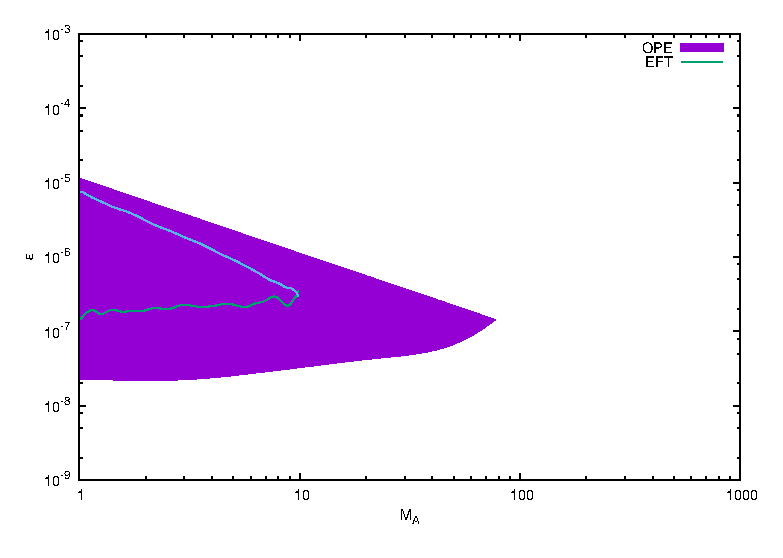
\includegraphics[height=9cm]{ope_bound.eps}
\caption{CAPTION}
\end{figure}

Both approaches produce constraints that are significantly weaker than the previous work, and that largely reproduce constraints already obtained from beam dump experiments. The squared matrix element obtained from the full one-pion-exchange in the end agrees quite well with that obtained using the approximations appropriate for axionic calculations; the reduction in the bremsstrahlung rate apparently results from significant changes to the phase space when the exact kinematics are used. The effective field theory calculation weakens the constraint by a further order of magnitude, and this difference between the EFT and OPE constraints results only from a difference in the matrix element calculated from each. It's well-known that the OPE model ignores effects related to chiral symmetry, and these evidently serve to reduce the bremsstrahlung rate considerably. Although there is some question as to the applicability of the simple pionless EFT at the highest masses considered, but at that point even significant deviation would not change the overall conclusion.

\section{Discussion/Conclusion}	
	
\acknowledgments

AKL was supported in part by NSF grant PHY-1519175.


\begin{thebibliography}{99}
%\normalsize

%\cite{Dent:2012mx}
\bibitem{Dent:2012mx} 
  J.~B.~Dent, F.~Ferrer and L.~M.~Krauss,
  %``Constraints on Light Hidden Sector Gauge Bosons from Supernova Cooling,''
  arXiv:1201.2683 [astro-ph.CO].
  %%CITATION = ARXIV:1201.2683;%%
  %56 citations counted in INSPIRE as of 29 Jul 2016


\end{thebibliography}


\end{document}

%%%%%%%%%%%%%%%%%%%%%%%%%%%%%%%%%%%%%%%%%%%%%%%%%%%%%%%%%%%%%%%%%%%%%%
%%%%%%%%%%%%%%%%%%%%%%%%%%%%% Bibliography %%%%%%%%%%%%%%%%%%%%%%%%%%%
%%%%%%%%%%%%%%%%%%%%%%%%%%%%%%%%%%%%%%%%%%%%%%%%%%%%%%%%%%%%%%%%%%%%%%


%%%%%%%%%%%%%%%%%%%%%%%%%%%%%%%%%%%%%%%%%%%%%%%%%%%%%%%%%%%%%%%%%%%%%%

\end{document}
